\documentclass[compress]{beamer}
\usepackage[francais]{babel}
\usepackage[latin1]{inputenc}
\usepackage{beamerthemesplit}
\usepackage[usenames,dvipsnames]{pstricks}
\usepackage{epsfig}
\usepackage{pst-grad} % For gradients
\usepackage{pst-plot} % For axes

\newcommand{\diapo}[2]{\frame{\frametitle{#1}#2}}
\newcommand{\imp}[1]{\textit{\textbf{#1}} }



\title{Carte de Kohonen}
\author{Hubert Godfroy}
\date{12 juin 2012\\ \texttt{https://github.com/hurlebouc/kohonen}}

\begin{document}

\frame{\titlepage}

\section[Plan]{}
\frame{\frametitle{Plan}\tableofcontents}

\section{Rappels}

\diapo{Rappels}{
\begin{itemize}
\item R�seau de neurones
	\begin{itemize}
	\item Fonction de transfert pour chaque neurone
	\item Relation entre les neurones
	\item Organisation du r�seau (couches)
	\end{itemize}
\item Apprentissage non-supervis�
	\begin{itemize}
	\item Le r�seau �volue seul en fonction des entr�es qui lui sont donn�es.
	\item Il modifie les poids des liaisons entre neurones.
	\end{itemize}
\end{itemize}
}

\diapo{Structure}{
	% !TEX root = ../presentation.tex

% Generated with LaTeXDraw 2.0.8
% Sat Jun 09 10:58:37 CEST 2012
% \usepackage[usenames,dvipsnames]{pstricks}
% \usepackage{epsfig}
% \usepackage{pst-grad} % For gradients
% \usepackage{pst-plot} % For axes
\scalebox{1} % Change this value to rescale the drawing.
{
\begin{pspicture}(0,-1.5)(10.129199,1.5)
\psframe[linewidth=0.04,dimen=outer](2.6,-0.7)(1.8,-1.5)
\psframe[linewidth=0.04,dimen=outer](1.4,-0.7)(0.6,-1.5)
\psframe[linewidth=0.04,dimen=outer](3.8,-0.7)(3.0,-1.5)
\psframe[linewidth=0.04,dimen=outer](5.0,-0.7)(4.2,-1.5)
\psframe[linewidth=0.04,dimen=outer](0.8,1.5)(0.0,0.7)
\psframe[linewidth=0.04,dimen=outer](2.0,1.5)(1.2,0.7)
\psframe[linewidth=0.04,dimen=outer](3.2,1.5)(2.4,0.7)
\psframe[linewidth=0.04,dimen=outer](4.4,1.5)(3.6,0.7)
\psframe[linewidth=0.04,dimen=outer](5.6,1.5)(4.8,0.7)
\psline[linewidth=0.04cm,linecolor=blue,arrowsize=0.05291667cm 2.0,arrowlength=1.4,arrowinset=0.4]{->}(1.6,0.7)(1.0,-0.7)
\psline[linewidth=0.04cm,linecolor=blue,arrowsize=0.05291667cm 2.0,arrowlength=1.4,arrowinset=0.4]{->}(0.4,0.7)(1.0,-0.7)
\psline[linewidth=0.04cm,linecolor=blue,arrowsize=0.05291667cm 2.0,arrowlength=1.4,arrowinset=0.4]{->}(0.4,0.7)(2.2,-0.7)
\psline[linewidth=0.04cm,linecolor=blue,arrowsize=0.05291667cm 2.0,arrowlength=1.4,arrowinset=0.4]{->}(0.4,0.7)(3.4,-0.7)
\psline[linewidth=0.04cm,linecolor=blue,arrowsize=0.05291667cm 2.0,arrowlength=1.4,arrowinset=0.4]{->}(0.4,0.7)(4.6,-0.7)
\psline[linewidth=0.04cm,linecolor=blue,arrowsize=0.05291667cm 2.0,arrowlength=1.4,arrowinset=0.4]{->}(1.6,0.7)(2.2,-0.7)
\psline[linewidth=0.04cm,linecolor=blue,arrowsize=0.05291667cm 2.0,arrowlength=1.4,arrowinset=0.4]{->}(1.6,0.7)(3.4,-0.7)
\psline[linewidth=0.04cm,linecolor=blue,arrowsize=0.05291667cm 2.0,arrowlength=1.4,arrowinset=0.4]{->}(1.6,0.7)(4.6,-0.7)
\psline[linewidth=0.04cm,linecolor=blue,arrowsize=0.05291667cm 2.0,arrowlength=1.4,arrowinset=0.4]{->}(2.8,0.7)(1.0,-0.7)
\psline[linewidth=0.04cm,linecolor=blue,arrowsize=0.05291667cm 2.0,arrowlength=1.4,arrowinset=0.4]{->}(2.8,0.7)(2.2,-0.7)
\psline[linewidth=0.04cm,linecolor=blue,arrowsize=0.05291667cm 2.0,arrowlength=1.4,arrowinset=0.4]{->}(2.8,0.7)(3.4,-0.7)
\psline[linewidth=0.04cm,linecolor=blue,arrowsize=0.05291667cm 2.0,arrowlength=1.4,arrowinset=0.4]{->}(2.8,0.7)(4.6,-0.7)
\psline[linewidth=0.04cm,linecolor=blue,arrowsize=0.05291667cm 2.0,arrowlength=1.4,arrowinset=0.4]{->}(4.0,0.7)(1.0,-0.7)
\psline[linewidth=0.04cm,linecolor=blue,arrowsize=0.05291667cm 2.0,arrowlength=1.4,arrowinset=0.4]{->}(4.0,0.7)(2.2,-0.7)
\psline[linewidth=0.04cm,linecolor=blue,arrowsize=0.05291667cm 2.0,arrowlength=1.4,arrowinset=0.4]{->}(4.0,0.7)(3.4,-0.7)
\psline[linewidth=0.04cm,linecolor=blue,arrowsize=0.05291667cm 2.0,arrowlength=1.4,arrowinset=0.4]{->}(4.0,0.7)(4.6,-0.7)
\psline[linewidth=0.04cm,linecolor=blue,arrowsize=0.05291667cm 2.0,arrowlength=1.4,arrowinset=0.4]{->}(5.2,0.7)(1.0,-0.7)
\psline[linewidth=0.04cm,linecolor=blue,arrowsize=0.05291667cm 2.0,arrowlength=1.4,arrowinset=0.4]{->}(5.2,0.7)(2.2,-0.7)
\psline[linewidth=0.04cm,linecolor=blue,arrowsize=0.05291667cm 2.0,arrowlength=1.4,arrowinset=0.4]{->}(5.2,0.7)(3.4,-0.7)
\psline[linewidth=0.04cm,linecolor=blue,arrowsize=0.05291667cm 2.0,arrowlength=1.4,arrowinset=0.4]{->}(5.2,0.7)(4.6,-0.7)
\put(7,-1.195){Couche d'entr�e}
\put(7 ,1.005){Carte de \textsc{Kohonen}}
\put(7 ,0.0050){Liaisons pond�r�es}
\end{pspicture} 
}


}

\diapo{Apprentissage}{
	\begin{itemize}
	\item Porte sur les neurones de la carte
	\item On rep�re le neurone \imp{vainqueur} qui est le plus "proche" de la couche d'entr�e au sens des poids.
	\item Ses poids sont modifi�s pour diminuer cette distance.
	\item Cette modification est propag�e aux neurones voisins du vainqueur.
	\end{itemize}
}

\section{Application}

\diapo{Application : ROC}{
	\begin{itemize}
	\item la couche d'entr�e est un agencement en 2 dimensions de neurone repr�sentant chacun un pixel de l'image.
	\item La carte de Kohonen est de dimension 2
	\item L'ensemble des poids d'un neurone de la carte peut �tre vu comme la moyenne des pixels ayant �t� vue par ce neurone. Chaque neurone est donc une moyenne d'image qu'il a rencontr�es.
	\end{itemize}
	\texttt{http://hurlebouc.github.com/kohonen/doc/inherits.html}
}

\diapo{Couche d'entr�e}{
\begin{figure}
\centering
\scalebox{0.7} % Change this value to rescale the drawing.
{
\begin{pspicture}(0,-3.9)(8.8,3.92)
\psframe[linewidth=0.04,dimen=outer](8.8,2.1)(2.8,-3.9)
\pscustom[linewidth=0.04]
{
\newpath
\moveto(6.8,1.5)
\lineto(6.3,1.3)
\curveto(6.05,1.2)(5.65,0.9)(5.5,0.7)
\curveto(5.35,0.5)(5.1,0.1)(5.0,-0.1)
\curveto(4.9,-0.3)(4.75,-0.7)(4.7,-0.9)
\curveto(4.65,-1.1)(4.7,-1.45)(4.8,-1.6)
\curveto(4.9,-1.75)(5.15,-2.0)(5.3,-2.1)
\curveto(5.45,-2.2)(5.85,-2.3)(6.1,-2.3)
\curveto(6.35,-2.3)(6.7,-2.1)(6.8,-1.9)
\curveto(6.9,-1.7)(6.95,-1.3)(6.9,-1.1)
\curveto(6.85,-0.9)(6.6,-0.55)(6.4,-0.4)
\curveto(6.2,-0.25)(5.8,-0.15)(5.6,-0.2)
\curveto(5.4,-0.25)(5.1,-0.4)(4.8,-0.7)
}
\psframe[linewidth=0.04,dimen=outer](3.4,2.1)(2.8,1.5)
\psframe[linewidth=0.04,dimen=outer](1.8,3.9)(0.0,2.1)
\psline[linewidth=0.04cm,linestyle=dotted,dotsep=0.16cm](2.8,1.5)(0.0,2.1)
\psline[linewidth=0.04cm,linestyle=dotted,dotsep=0.16cm](3.4,1.5)(1.8,2.1)
\psline[linewidth=0.04cm,linestyle=dotted,dotsep=0.16cm](3.4,2.1)(1.8,3.9)
\psline[linewidth=0.04cm,linestyle=dotted,dotsep=0.16cm](2.8,2.1)(0.0,3.9)
\usefont{T1}{ptm}{m}{n}
\rput(0.96964353,3.205){\small neurone}
\usefont{T1}{ptm}{m}{n}
\rput(0.9625,2.805){\small input}
\end{pspicture} 
}
\caption{Repr�sentation de la couche d'entr�e}
\end{figure}
}

\diapo{Repr�sentation de la carte}{
Les poids repr�sentent les niveaux de gris
\begin{figure}
\centering
\scalebox{1} % Change this value to rescale the drawing.
{
\begin{pspicture}(0,-1.52)(3.02,1.52)
\psframe[linewidth=0.04,dimen=outer](3.0,1.5)(0.0,-1.5)
\psline[linewidth=0.04cm](1.0,1.5)(1.0,-1.5)
\psline[linewidth=0.04cm](2.0,1.5)(2.0,-1.5)
\psline[linewidth=0.04cm](0.0,0.5)(3.0,0.5)
\psline[linewidth=0.04cm](0.0,-0.5)(3.0,-0.5)
\usefont{T1}{ptm}{m}{n}
\rput(0.43145508,1.005){$n_1$}
\usefont{T1}{ptm}{m}{n}
\rput(1.4314551,1.005){$n_2$}
\usefont{T1}{ptm}{m}{n}
\rput(2.4314551,1.005){$n_3$}
\usefont{T1}{ptm}{m}{n}
\rput(0.43145508,0.0050){$n_4$}
\usefont{T1}{ptm}{m}{n}
\rput(1.4314551,0.0050){$n_5$}
\usefont{T1}{ptm}{m}{n}
\rput(2.4314551,0.0050){$n_6$}
\usefont{T1}{ptm}{m}{n}
\rput(0.43145508,-0.995){$n_7$}
\usefont{T1}{ptm}{m}{n}
\rput(1.4314551,-0.995){$n_8$}
\usefont{T1}{ptm}{m}{n}
\rput(2.4314551,-0.995){$n_9$}
\end{pspicture} 
}
\caption{Repr�sentation de la couche de \textsc{Kohonen}}
\end{figure}

}

\diapo{Exemple}{
	\begin{figure}[htbp]
	\centering
	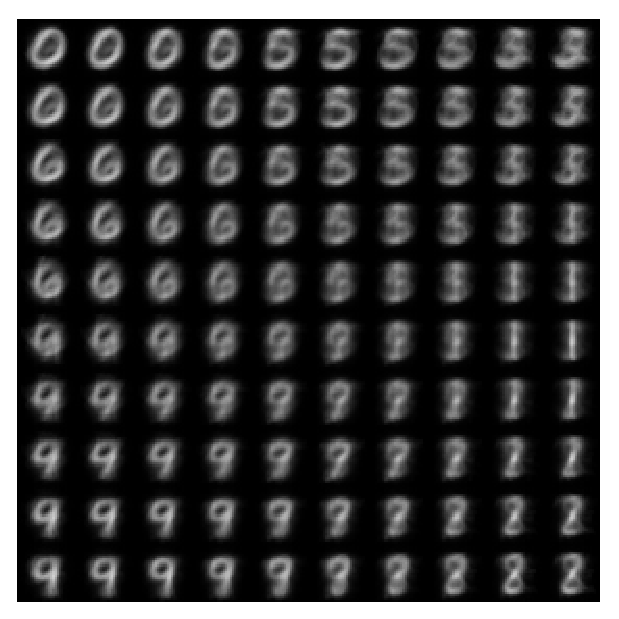
\includegraphics[width=5cm]{images/res.eps}
	\caption{Carte de \textsc{Kohonen} apr�s apprentissage}
	\end{figure}
}

\section{Discussion}

\diapo{Discussion}{
	\begin{itemize}
	\item Comment utiliser cette carte dans la ROC ?
	\item Comment �tablir un classement ?
	\end{itemize}
}

\diapo{S�lection des classes par �tude des fr�quences}{
	\begin{figure}
		\centering
		
\includegraphics[width=5cm]{images/freq.eps}
		\caption{Repr�sentation des fr�quences}
	\end{figure}
}

\diapo{Interpr�tation}{
	\begin{itemize}
	\item Les r�f�rences sont les maxima locaux.
	\item Les classes sont obtenues � partir d'un diagramme de \textsc{Voronoi}.
	\end{itemize}
}

\diapo{Classification}{
	\begin{figure}
		\centering
		
\includegraphics[width=5cm]{images/classe.eps}
		\caption{Diagramme de \textsc{Voronoi}}
	\end{figure}
}

\diapo{Assembl�e d�cisionnelle}{

\begin{figure}
\centering
\scalebox{0.8} % Change this value to rescale the drawing.
{
\begin{pspicture}(0,-2.82)(6.82,2.82)
\psline[linewidth=0.04cm](0.0,1.6)(1.8,1.6)
\psline[linewidth=0.04cm](1.2,2.8)(3.0,2.8)
\psline[linewidth=0.04cm](1.2,2.8)(0.0,1.6)
\psline[linewidth=0.04cm](1.8,2.8)(0.6,1.6)
\psline[linewidth=0.04cm](1.2,1.6)(2.4,2.8)
\psline[linewidth=0.04cm](1.8,1.6)(3.0,2.8)
\psline[linewidth=0.04cm](0.8,2.4)(2.6,2.4)
\psline[linewidth=0.04cm](0.4,2.0)(2.2,2.0)
\psline[linewidth=0.04cm](3.8,1.6)(5.6,1.6)
\psline[linewidth=0.04cm](5.0,2.8)(6.8,2.8)
\psline[linewidth=0.04cm](5.0,2.8)(3.8,1.6)
\psline[linewidth=0.04cm](5.6,2.8)(4.4,1.6)
\psline[linewidth=0.04cm](5.0,1.6)(6.2,2.8)
\psline[linewidth=0.04cm](5.6,1.6)(6.8,2.8)
\psline[linewidth=0.04cm](4.6,2.4)(6.4,2.4)
\psline[linewidth=0.04cm](4.2,2.0)(6.0,2.0)
\psline[linewidth=0.04cm](1.0,-0.4)(2.8,-0.4)
\psline[linewidth=0.04cm](2.2,0.8)(4.0,0.8)
\psline[linewidth=0.04cm](2.2,0.8)(1.0,-0.4)
\psline[linewidth=0.04cm](2.8,0.8)(1.6,-0.4)
\psline[linewidth=0.04cm](2.2,-0.4)(3.4,0.8)
\psline[linewidth=0.04cm](2.8,-0.4)(4.0,0.8)
\psline[linewidth=0.04cm](1.8,0.4)(3.6,0.4)
\psline[linewidth=0.04cm](1.4,0.0)(3.2,0.0)
\psline[linewidth=0.04cm](1.4,-2.8)(3.2,-2.8)
\psline[linewidth=0.04cm](2.6,-1.6)(4.4,-1.6)
\psline[linewidth=0.04cm](2.6,-1.6)(1.4,-2.8)
\psline[linewidth=0.04cm](3.2,-2.8)(4.4,-1.6)
\psline[linewidth=0.04cm,arrowsize=0.05291667cm 2.0,arrowlength=1.4,arrowinset=0.4]{->}(2.8,-2.2)(2.2,-0.4)
\psline[linewidth=0.04cm,arrowsize=0.05291667cm 2.0,arrowlength=1.4,arrowinset=0.4]{->}(2.8,-2.2)(5.0,1.6)
\psline[linewidth=0.04cm,arrowsize=0.05291667cm 2.0,arrowlength=1.4,arrowinset=0.4]{->}(2.8,-2.2)(1.0,1.6)
\end{pspicture} 
}
\caption{Processus de d�cision}
\end{figure}

}







\end{document}
